\chapter[Documento de Visão]{Documento de Visão}

\section{Introdução}
A finalidade deste documento é coletar, analisar e definir necessidades e recursos de nível superior do CIAC. Ele se concentra nos recursos necessários aos envolvidos e aos usuários-alvo e nas razões que levam a essas necessidades. Os detalhes de como o CIAC satisfaz essas necessidades são descritos nas especificações de requisitos.

\subsection{Finalidade}
Este documento tem a finalide de  esclarecer e possibilitar uma visão do sistema que será uma informação importante para o entendimentos dos envolvidos no projeto.
\subsection{Escopo}
Este está inserido em um contexto de especificação dos usuários que estarão utilizando o sistema, os interessados no projeto, os requisitos não funcionais, sistemas semelhantes, recursos e características. Bem como a indicação da documentação que será desenvolvida para auxílio dos usuários ao utilizar o sistema.
\subsection{Visão Geral}
Este documento está dividido em doze sessões, descrevendo o Posiconamento do Projeto, Usuários, Visão Geral do Produto, Recursos do Produto, Restrições, Intervalos de Qualidade, Outros Requisitos do Produto, Requisitos de Documentação, Análise dos Softwares Semelhantes, Desenvolver, Comprar ou Customizar? e por fim, Subsistemas que o CIAC possui.

\section{Posicionamento}

\subsection{Oportunidade de Negócios}
Dado o grande numero de acidentes que ocorrem no Brasil, percebe-se que com o
desenvolvimento de um sistema de alerta na ultrapassagem, pode-se obter
ganhos ao evitar gastos com as consequências dos acidentes para todos os
brasileiros usuários das rodovias. Dado que, segundo a PRF, o tipo de acidente
que mais mata é a colisão frontal, causada, especialmente, pelas ultrapassagens
forçadas ou em locais sem visibilidade\cite{prf}.

A maioria dos acidentes ocorre a luz do dia, em pistas de mão única, com tempo bom. O estudo do Instituto de Pesquisa
Econômica e Aplicada (IPEA), do ministério do Planejamento, mostra que menos da metade dos acidentes acontecem em estradas
de mão dupla. O índice à noite não chega a 40\%, e em apenas 20\% dos casos estava chovendo. A pesquisa mostra ainda que o
 cansaço nem sempre é o responsável. Os acidentes mais freqüentes são com motoristas dirigindo há no máximo uma hora.
 Segundo a Polícia Rodoviária Federal, é a imprudência a principal causa \cite{acidentesDeTransitoNoBrasil}

 Considerando a mortalidade por tipo de acidente, lideram a condição de maior gravidade os acidentes do tipo colisão
 frontal, com 24,6\% das mortes. Muito embora esses tipos de acidentes representem apenas 4,0\% das ocorrências é o que
 possui característica mais letal — a cada 100 acidentes desse tipo, morrem 33,23 pessoas. Colisões frontais — fato que
 seria esperado, pois são acidentes que ocorrem, na grande maioria deles, em vias com pista simples, com envolvimento de
 veículos em velocidade. \cite{custos_acidentes_transito}

 Cerca de 90\% (81,75\%) das colisões frontais, como era de se esperar, ocorreram em pista simples, com
 tráfego nos dois sentidos, sem separação física dos fluxos opostos. Análise dos dados sobre os 10\% que
 ocorreram em pista dupla revela participação significativa, mas não exclusiva, de bicicletas e motocicletas,
 circulando provavelmente na contramão. Segundo os dados analisados, algumas colisões frontais ocorreram em
 curvas em vias de pista dupla. Essas características sugerem algumas situações prováveis de ocorrência das
 colisões frontais, a serem verificadas ou não nas vistorias, conforme a seguir descrito. \cite{fatoresCondicionantesGravidade}

 Em pista simples:

 • ultrapassagem de veículos pesados e lentos em trechos em aclive, especialmente
em condições de congestionamento;

 • ultrapassagem indevida em geral; e

 • problemas de falta de visibilidade.

 Em pista dupla:

 • veículos transitando na contramão, especialmente bicicletas e motocicletas; e

 • curvas fechadas e/ou com superelevação insuficiente e/ou sem barreira/defensa
 no canteiro central.


O número de vítimas no trânsito brasileiro é o maior do mundo. De acordo com o Levantamento do Observatório
 Nacional de Segurança Viária, divulgado pela revista Veja desta semana, os acidentes de carro superam
 homicídios ou câncer, por exemplo. Segundo registro no seguro DPVAT (Danos Pessoais Causados por Veículos
  Automotores de Via Terrestre), o país tem 31,3 vítimas fatais por 100 mil habitantes; mais que o
  verificado no Catar, El Salvador, Belize e Venezuela.\cite{brasilTemMaisVitimasDeTransito}


\subsection{Descrição do Problema}
\begin{table}[ht]
\caption{Framework do Problema}
\centering
\begin{tabular}{| l |  p{7cm} |}
\hline
O problema da & Grande quantidade de acidentes, cuminando em mortes, que acontecem nas rodovias brasileiras devido a execução de ultrapassagens mal sucedidas.  \\
\hline
Afeta & O povo brasileiro que é usuário das rodovias como meio de transporte. \\
\hline
Cujo o impacto é & A Morte de vários brasileiros, bem como a perca de bens materiais no momento do acidente.\\
\hline
Uma boa solucao seria & A Implementação de um sistema que possibilite a sinalização ao motorista sobre quando e possivel executar a ultrapassagem. \\
\hline
\end{tabular}
\end{table}


\subsection{Sentença de Posição do Produto}

\begin{table}[ht]
\caption{Designação do Produto}
\centering
\begin{tabular}{| l |  p{7cm} |}
\hline
Para & Brasileiros que utilizam as rodovias como meio de locomoção a partir de qualquer automóvel. \\
\hline
Que & Evitará os acidentes no momento que os usuários das rodovias forem executar ultrapassagens. \\
\hline
O CIAC & É uma categoria de sistenas de segurança\\
\hline
Que & Culminará na queda dos indicares de mortalidade devido a acidentes de transito nas rodovias decorrentes de ultrapassagens \\
\hline
Diferente de & Produtos pré instalados em carros adquiridos em concenssonárias e que não são fornecidos no Brasil.  \\
\hline
Nosso Produto & Pode ser adiquirido por qualquer motorista para qualquer automóvel no Brasil\\
\hline
\end{tabular}
\end{table}

\section{Estrutura Analítica de Projetos}
Para o nosso projeto, traçamos uma Estrutura Analítica de Projetos (EAP) com o objetivo de deixar claro o nosso
desenvolvimento orientado aos pontos de controle, bem como os objetivos que iremos alcançar em cada etapa.


\begin{figure}[h]
  \centering
  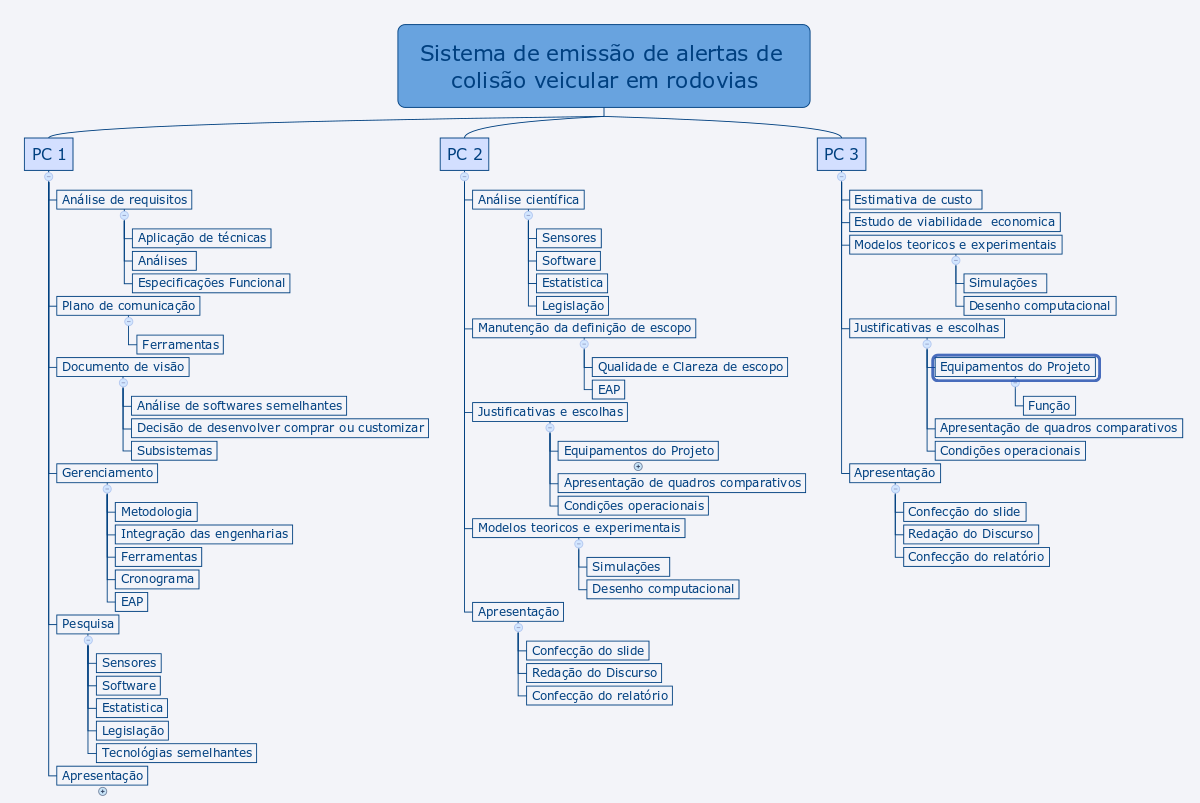
\includegraphics[width=450px, scale=0.5]{figuras/eap}
  \caption{Estrutura Analítica de Projetos}
  \label{fig:eap}
\end{figure}

\section{Descrições dos Envolvidos e dos Usuários}

\subsection{Perfil dos Usuários}
O perfil do público alvo desejado pelos integrantes do projeto é o de qualquer cidadão que possua carteira de motorista reconhecida em território nacional, de acordo com o Código de Trânsito Brasileiro\cite{ctb}.

\subsection{Ambiente do Usuário}
O ambiente de uso do sistema será as rodovias brasileiras. O sistema estará instalado no carro do usuário e emitirá os devidos alertas ao mesmo de acordo com as especificações que serão abordadas neste relatório.

\subsection{Perfil dos Envolvidos}
Os envolvidos na elaboração/idealização técnica do produto são os alunos graduandos da Universidade de Brasília - Faculdade do Gama cursando a disciplina de Projeto Integrador.

\section{Recursos do Produto}
Os tópicos a seguir ilustrarão quais as capacidades do nosso sistema.
\subsection{Acionamento da verificação de segurança}
O motorista poderá acionar o sistema de segurança ao ter a intenção de ultrapassar.
Quando este acionar o sistema através de alguma entrada, será executado o algorítimo para a verificação da possibilidade de
ultrapassagem, analisando se o caminho a ser percorrido para ultrapassar está em condições desejávies, isto é,
se não há nenhum outro carro vindo na direção oposta em codição de colisão.

\subsection{Alerta de Perigo}
Ao analisar a possibilidade de ultrapassagem, o sistema irá alertar ao motorista caso esta seja insegura.

\section{Restrições}
Devido a quantidade de acidentes decorridos de ultrapassagens ser maior em rodovias, nosso sistema tera a restriçao de atender apenas os usuarios transitando nestes locais. Alem disso, o trafico de automoveis em todas as direcoes e muito alto, cuminando assim na ineficiencia do sistema ao detectar a todo momento que a ultrapassagem e inadequada.

Dessa maneira, a utilizacao do projeto dentro de cidades nao viavel, possibilitando o uso apenas em rodivias.

\section{Requisitos de Documentação}
Esta seção descreve a documentação que deverá ser desenvolvida para suportar a implantação bem-sucedida de aplicativos.

\subsection{Manual do Usuário}
O sitema contera dentro da embalagem a ser adquirida um manual de instruçoes de uso do sistema, bem como orientaçoes sobre instalacao e manutencao.

\subsection{Ajuda On-line}
Sera disponibilizada uma documentacao online para auxilio do usuario em qualquer aspecto de uso. Serao disponibilizados os manuais fisicos, esta documentacao de desenvolvimento do projeto como: Documento de Visao, Especificaçao dos Requisitos e Prototipos de Tela

\section{Análise dos Softwares Semelhantes}
Recentemente, vários dispositivos anti-colisão têm sido projetados e lançados, entretanto ainda não foi feito um dispositivo com o intuito
de prevenir colisões durante ultrapassagem. A Volvo, por exemplo, desenvolveu um dispositivo de segurança que prevê rotas em situação de
colisão. O sistema possui sensores que permitem monitoramento de 360º ao redor do carro, aprimorado por um gerador de manobra, freio ou controle
automático da direção, um software que identifica possíveis rotas de fuga. Para isso, se fez necessário o desenvolvimento de uma estrutura central
que reúne vários sensores, a fim de permitir que câmeras, radares por ondas, radares por laser e GPS trabalhem em conjunto \cite{volvo}. A
 Figura \ref{fig:sistemavolvo} ilustra
 o sistema lançado pela empresa.

 \begin{figure}[h]
   \centering

   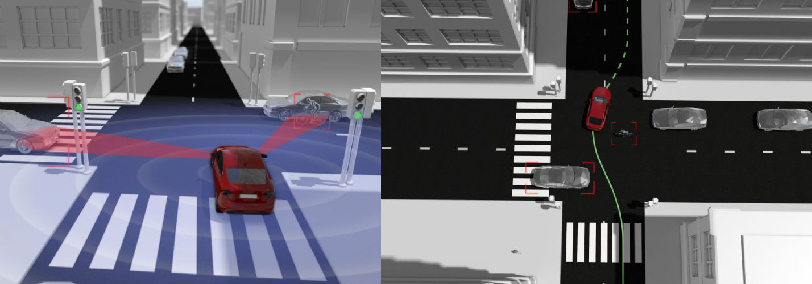
\includegraphics[width=450px, scale=1]{figuras/sistemavolvo}
   \caption{Ilustração do Sistema anti-colisão da Volvo}

\label{fig:sistemavolvo}
 \end{figure}


Outro dispositivo com aplicação semelhante é o da empresa Distritec, que é um sistema anti-colisão que detecta pessoas e objetos, que possui
um sensor de detecção, um display montado na cabine do veículo, tecnologia de radar por pulsos que alerta o usuário quando há algum obstáculo
 parado ou em movimento em uma área pré-definida de 10 metros. O sistema não precisa de limpeza, não é afetado por condições climáticas adversas
  \cite{distritec}.

O dispositivo que foi desenvolvido em um projeto de pesquisa da universidade Mauá, apresenta um sistema de navegação para veículo baseado na
transmissão de dados entre veículos. O sistema utiliza parâmetros estimados para determinar a velocidade e posição relativa de veículos autônomos
e módulos com tecnologia para permitir a comunicação entre veículos e estimar a distância entre os veículos por meio de um algoritmo \cite{sensoriamento}.

Foi feita uma abordagem simples desse tipo de sistema, através de um microcontrolador, um sensor de velocidade e um sensor de distância. O sistema
 pode ser utilizado em vários veículos, com alterações em sua programação, que é feita com liguagem C. O circuito eletrônico é capaz de alertar o
 condutor de um veículo, a qualquer risco eminente de colisão a pouco mais de 6,3 metros, com velocidade máxima de 7 km/h, aproximadamente \cite{iesam}.

A Chevrolet também laçou um sistema anti-colisão, com funcionamento semelhante ao recurso oferecido por outras marcas, porém com apenas uma câmera
 que faz a identificação de eventuais obstáculos à frente, o dispositivo alerta o motorista sobre perigos e freia o veículo automaticamente para
 evitar impactos, assim como o dispositivo lançado pela Volvo, já citado. A General Motors busca popularizar a tecnologia e aplicá-la também nos
 carros mais baratos do portfólio. O sistema é capaz de frear o veículo a velocidades de até 25 km/h \cite{chevrolet}.

 A Toyota também lançou um modulo de prevenção de colisões, o Pre-Collision System (PCS), que utiliza um sistema de sensores instalados na
 dianteira, que detecta a presença de pedestres, obstáculos ou outros automóveis, radares e câmeras especiais que permitem o cálculo da intensidade
  da frenagem e do movimento da direção necessários para escapar dos perigos da pista. O sistema emite luzes próximas ao infravermelho, com o
  objetivo de melhorar a visibilidade do motorista à noite \cite{toyota}.

 Foi projetado também um sistema constituído de dois alto-falantes localizados próximos a cabeça do motorista e de elementos vibratórios no
 acento, que são acionados por meio de sensores localizados ao redor do carro, o sistema é constituído por dois módulos, o módulo ativação
 identifica a situação de risco e informa ao módulo de alerta, que faz a ativação dos estímulos \cite{usp}. A Figura \ref{fig:sistemaanticolisao} ilustra os módulos do sistema.


  \begin{figure}[h]
    \centering
    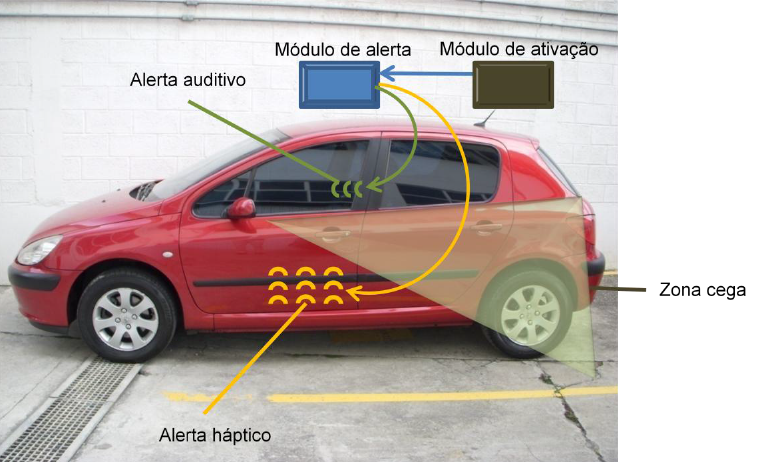
\includegraphics[width=400px, scale=0.5]{figuras/sistemaanticolisao}
    \caption{Esquemático do Sistema anti-colisão}
    \label{fig:sistemaanticolisao}
  \end{figure}

\subsection{City Safety}
Este sistema tem como objetivo reduzir os estragos de acidentes. Ao detectar que seu carro se aproxima intensamente de outro veículo sem que o pedal do freio seja utilizado, o City Safety se encarrega de frear o veículo automaticamente. Ele evita colisões a baixas velocidades e se faz efetivo somente quando a diferença máxima de velocidade entre os veículos é de 30 Km/h.

Em condições ideais, o City Safety evita completamente colisões até diferença de velocidade de 15 km/h, já entre 15 e 30 km/h o impacto será reduzido drasticamente. Ele é acionado ao se deparar com veículos no mesmo sentido ou ainda com objetos estáticos, lembrando que é possível mudar de faixa durante o tráfego pesado, sem a intervenção do sistema.

O sistema pode ser desabilitado através do controle do painel. Próximo do espelho retrovisor interno, dentro do pára-brisa, localiza-se um sensor a laser que reconhece objetos até 10 m à frente do pára-choque do veículo. Ele é o responsável pelo monitoramento do tráfego e pela ativação do freio, mas somente em casos extremos.

Trata-se de um acessório que evita colisões em momentos críticos, portanto deve ser utilizado como tal. É necessário respeitar as regras vigentes nas leis de trânsito.

A luminosidade não interfere na funcionalidade do sistema. Dirigir sob neblina, chuva ou neve intensa limita o funcionamento do sistema.

\subsection{Toyota}
O sitema anti colisão da toyota é um conjunto sub sistemas que prometem alertar o motorista em diferentes situações que podem ocasionar colisões. A solução proposta por eles pretendem garantir a segurança: ao estacionar; segurança ativa que previne acidentes, sistema que previne colisões, um sistema passivo que protege o usuário, e um sistema de resposta a chamadas de emergência.

Diferentemente da proposta do nosso projeto, a toyota atuará sobre os comandos do carro, com um sistema de controle de estabilidade, assistência na frenagem. Além disso, possuirá subsistema para auxílio ao estacionar, identificação de pedestres, auxiliar a visão noturna, e ativar um chamado automático dos socorristas em casos de acidentes \cite{toyota}.

\begin{figure}[h]
  \centering
  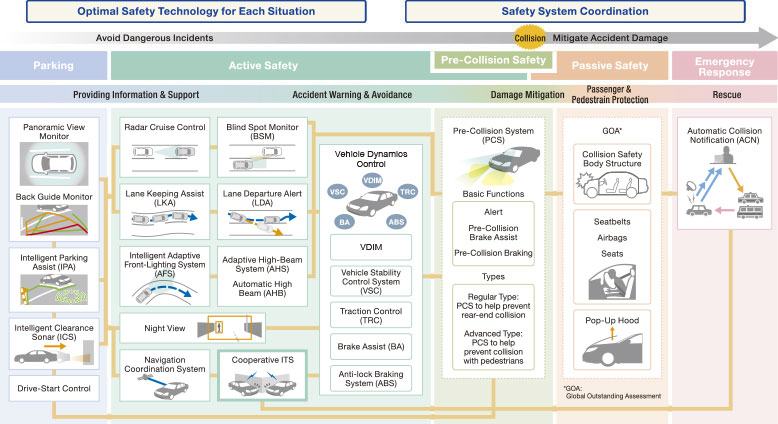
\includegraphics[width=450px, scale=0.5]{figuras/sistematoyota}
  \caption{Sistema de auxilio da Toyota}
  \label{fig:sistematoyota}
\end{figure}

A Figura \ref{fig:sistematoyota} trás um diagrama do sistema como um todo projetado por eles. Percebe-se que há várias funcionalidades complementares umas as outras, mas que estão separadas em diferentes níveis. A toyota projetou de forma que o sistema contempla a prevenção de acidentes até a segurança do motorista caso o acidente ocorra.

\subsection{Ford - Tecnologia de Assistência ao Motorista e Prevenção de Acidentes}
A Ford vem desenvolvendo um sistema que tem várias funções de auxílio ao motorista e de prevenção de acidentes, entre elas, um dispositivo que avisa ao condutor sobre uma possível colisão.

A tecnologia em questão difere da proposta pelo nosso projeto, pois ela é semi-automatizada e atua da seguinte forma: em caso de um alto de risco de colisão com o veículo da frente, o sistema emite alertas audiovisuais, e ele possui um dispositivo chamado “servo boost” que, em caso do condutor retirar o pé do acelerador ele já deixa o freio programado para proporcionar um desempenho mais rápido ao condutor. Se o sistema apresentar alguma falha e/ou tiver sua funcionalidade reduzida, o sistema apresenta um alerta para o condutor.

\begin{figure}[h]
  \centering
  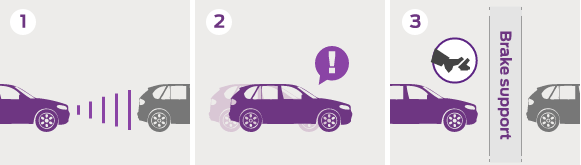
\includegraphics[width=450px, scale=0.5]{figuras/sistemaford}
  \caption{Alerta do veículo}
  \label{fig:sistemaford}
\end{figure}

\subsection{Anti collision warning system AWS650}
AWS é usado principalmente na estrada , via expressa urbana e outra estrada de alta qualidade. O seu principal objetivo é ajudar o condutor a manter-se na pista e manter a distância, evitar acidentes de trânsito e ao mesmo tempo , reduzindo o risco de acidente de colisão frontal causada por distração do condutor , de modo a reduzir a lesões.

O produto combina identificação de imagem , estimativa de risco e muitas tecnologias de ponta, completamente cumprimento das condição rodoviárias internacional, as leis de trânsito e do hábito do motorista. Quando o veículo passivamente sair da pista devido à distração ou cansaço do condutor , chegar muito perto com o carro da frente, ou há outro veículo ultrapassando em curta distância , o sistema automaticamente aciona o alarme até que o motorista corrija a direção de condução ou controlar ativamente a distância do  veículo.

O sistema só tem a função de lembrança da segurança, o mesmo não tomará automaticamente medidas para intervir operação do motorista. O motorista ainda deve ser responsável pela segurança de condução.

\begin{figure}[h]
  \centering
  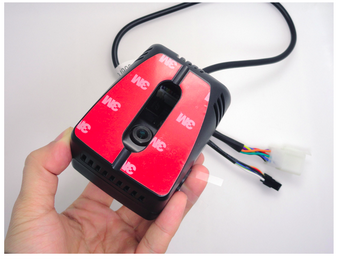
\includegraphics[width=300px, scale=0.5]{figuras/sensoraws650}
  \caption{Sensor aws650}
  \label{fig:sensoraws650}
\end{figure}

Quando o veículo está inconscientemente saindo da pista de condução, irá fornecer um forte alarme para o motorista até que ele corrija a direção. O seu objetivo é o de evitar o acidente que causou pelo cansaço ou distração do motorista para inconscientemente saída da pista. Seu princípio é reconhecer e acompanhar sua posição à pista o mais próximo do veículo da frente, a câmera frontal , em tempo real calcula a distância entre a faixa da esquerda da  pista da direita e roda dianteira do veículo.

\begin{figure}[h]
  \centering
  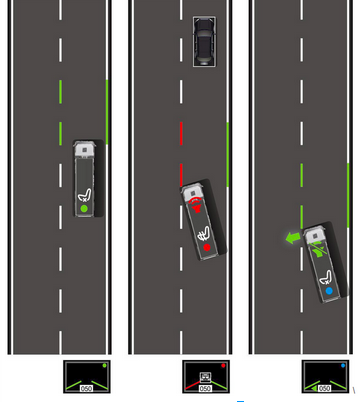
\includegraphics[width=300px, scale=0.5]{figuras/situacaoPerigo}
  \caption{Situação de utilização do aws650}
  \label{fig:situacaoPerigo}
\end{figure}

\subsection{Forward Collision Warning}
Leva a câmera como principal sensor, detectação de trilhas do veículo da frente em cima da tecnologia visual da máquina , que combina as características do motorista para julgar se o veículo está muito perto do veículo da frente, fornecendo aviso de som e luminoso para os motoristas.
Quando o veículo está demasiadamente próximo do veículo da frente ou tem perigo de colisão, o sistema irá fornecer um toque alarmante, para avisar aos pilotos para que que haja uma tomar de medidas para evitar o acidente repentino, reduzindo assim os acidentes de trânsito.

\begin{figure}[h]
  \centering
  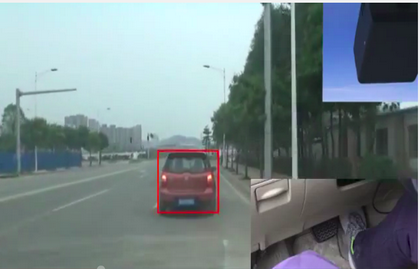
\includegraphics[width=300px, scale=0.5]{figuras/fowordCollision}
  \caption{Identificação realizada pela câmera do foword collision warning}
  \label{fig:fowordCollision}
\end{figure}


\begin{figure}[h]
  \centering
  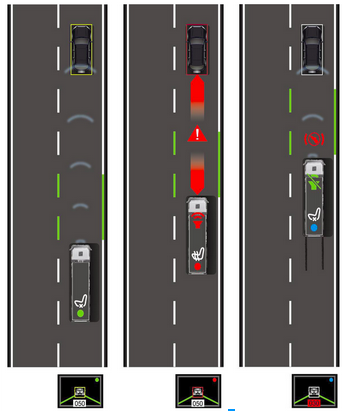
\includegraphics[width=300px, scale=0.5]{figuras/situacaoForwardCollision}
  \caption{Situação de funcionamento do forward collision warning}
  \label{fig:situacaoForwardCollision}
\end{figure}

\subsubsection{Especificações do Produto}

\begin{figure}[h]
  \centering
  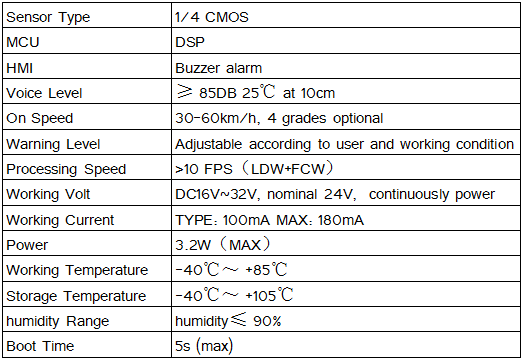
\includegraphics[width=300px, scale=0.5]{figuras/especificacaiForwardCollision}
  \caption{Situação de funcionamento do forward collision warning}
  \label{table:especificacaiForwardCollision}
\end{figure}

\section{Desenvolver, Comprar ou Customizar?}

\section{Subsistemas}
